 
\PassOptionsToPackage{ELEC}{aaltologo}
\documentclass[logo=bluequo,normaltitle]{aaltoslides}
%\documentclass{aaltoslides} % DEFAULT
%\documentclass[first=purple,second=lgreen,logo=bquo,normaltitle,nofoot]{aaltoslides} % SOME OPTION EXAMPLES

\usepackage[utf8]{inputenc}
\usepackage[T1]{fontenc}
\usepackage{graphicx}
\usepackage{amssymb,amsmath}
\usepackage{url}
\usepackage{lastpage}
\usepackage{epstopdf}
%\usepackage[pdfpagemode=None,colorlinks=true,urlcolor=red, linkcolor=black,citecolor=black,pdfstartview=FitH]{hyperref}
\usepackage{mdframed}
\usepackage{caption}
\usepackage{apacite}
\usepackage{tikz}
\usetikzlibrary{positioning,shapes,shadows,arrows}
\tikzset{
  every overlay node/.style={
    %draw=black,fill=white,rounded corners,
    anchor=north west, inner sep=0pt,
  },
  thick/.style=      {line width=0.3mm},
}
\def\tikzoverlay{%
   \tikz[remember picture, overlay]\node[every overlay node]
}%

%%%% This for easy placemnet of figure inside a block
\newcommand{\putfig}[3][1.0]{
    \begin{block}{#3}
        \includegraphics[width=#1\linewidth,height=#1\textheight,keepaspectratio]{#2}
    \end{block}
}
%%%%

%%%% To insert lecture date
\newcommand{\lectdate}{19.11.2015}
%%%%

\title{Example Beamer slide set with some fancy features}

\author[Marko Kosunen]{Marko Kosunen}
\institute[MNT]{Department of Micro and Nanosciences\\
Aalto University, School of Electrical Engineering\\marko.kosunen@aalto.fi}

\aaltofootertext{THIS IS THE FOOTER}{\lectdate}{\arabic{page}/\pageref{LastPage}\ }

\date{\lectdate}

\newcommand{\tellipse}[4]{
    \begin{tikzpicture}[overlay]
        \draw[secondarycolor,thick] (#1,#2) ellipse (#3 and #4);
    \end{tikzpicture}
}

\newcommand{\tarrow}[2]{
    \begin{tikzpicture}[overlay]
        \draw[secondarycolor,thick,->] (#1) -- (#2);
    \end{tikzpicture}
}
\begin{document}

%%%%%%%%%%%%%%%%%%%%%%%%%%%%%%%%%%%%%%%%%%%%%%%%%%%%%%%%%%%%%%%%%%%%%%%%%%%%%%%%%%%%%%%%%%%%%
% Generates the titleframe
\aaltotitleframe
%%%%%%%%%%%%%%%%%%%%%%%%%%%%%%%%%%%%%%%%%%%%%%%%%%%%%%%%%%%%%%%%%%%%%%%%%%%%%%%%%%%%%%%%%%%%%



%\AtBeginSection[]
%{
%%%Outlineframe
%    \begin{frame}{Outline}
%        \tableofcontents[currentsection]
%\end{frame}
%}
%\section*{Outline}
%\begin{frame}[t]
%        \tableofcontents
%\end{frame}


%%%%%%%%%%%%%%%%%%%%%%%%%%%%%%%%%%%%%%%%%%
\begin{frame}[t]
    \frametitle{Objective}
    \begin{itemize}
        \item Useful can insert useful slide structures by reading in one of the
            files TXXX.tex
            \pause
        \item Try them out to see if you like them        
    \end{itemize}
    %examples of ellipse and arrow
    \tellipse{0}{0}{2cm}{2cm}
    \tarrow{0,0}{2,2}
\end{frame}


%%%%%%%%%%%%%%%%%%%%%%%%%%%%%%%%%%%%%%%%%%
\begin{frame}[t]
    \frametitle{What is Digital?}
    \begin{itemize}
        \item<1-> Digital means quite literally ''numerical, and what we can say
            for sure, is that
            \begin{itemize}
                \item<2-> Analog information is continuous in time.
                \item<2-> Digital information is quantized and interpreted as a number).
            \end{itemize}
    \end{itemize}
     \includegraphics[width=0.7\textwidth]{./Pics/ADconvert.eps}\ 
\end{frame}


%%%%%%%%%%%%%%%%%%%%%%%%%%%%%%%%%%%%%%%%%%
% This slide contais a nice example of tikz for graphics. You use them for
% arrows etc
\begin{frame}[t]
    \frametitle{Some Tikz and overlay stuff}
    \begin{itemize}
            \pause
        \item  To put it simply: Computing
            \pause
        \item History of digital electronics is history of automated
            computing.
            \pause
        \item Number is very interference tolerant. 
            \pause
        \item We have (some) control over the
            noise and interference.
            \pause
    \end{itemize}
\begin{minipage}{.48\linewidth}
            \begin{center}
                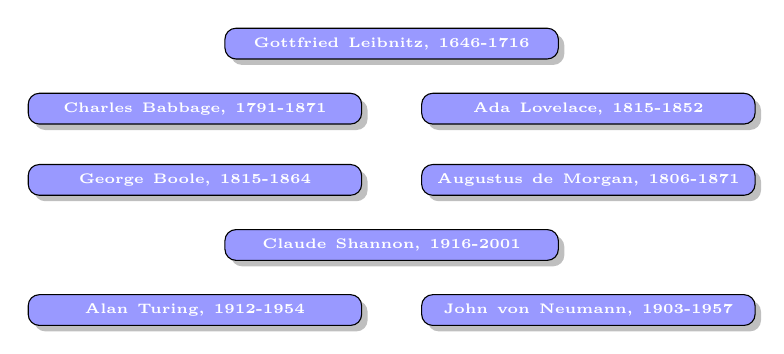
\begin{tikzpicture}
                    \tikzstyle{item}=[rectangle, draw=black, rounded corners, 
                        fill=blue!40, drop shadow,
                        text centered, anchor=north, text=white, text
                    width=4.0cm]
                    \node (Leibnitz) [item, rectangle]
                        {
                            \textbf{\tiny Gottfried Leibnitz, 1646-1716}
                        }; 

                        \node(Null1) [below= 0.5cm of Leibnitz]{};
                        \node (Babbage) [item, rectangle, left= 0.25cm of Null1]
                        {
                            \textbf{\tiny Charles Babbage, 1791-1871}
                        }; 

                        \node (Lovelace) [item, rectangle, right= 0.25cm of
                        Null1]
                        {
                            \textbf{\tiny Ada Lovelace, 1815-1852}
                        }; 
                        \node (Boole) [item, rectangle, below= 0.5cm of
                        Babbage]
                        {
                            \textbf{\tiny George Boole, 1815-1864}
                        }; 
                        \node (Morgan) [item, rectangle, below= 0.5cm of
                        Lovelace]
                        {
                            \textbf{\tiny Augustus de Morgan, 1806-1871}
                        }; 

                        \node(Null2) [right= 0.25cm of Boole]{};
                        \node (Shannon) [item, rectangle, below= 0.5cm of
                        Null2]
                        {
                            \textbf{\tiny Claude Shannon, 1916-2001}
                        }; 
                        \node(Null3) [below= 0.5cm of Shannon]{};
                        \node (Turing) [item, rectangle, left= 0.25cm of
                        Null3]
                        {
                            \textbf{\tiny Alan Turing, 1912-1954}
                        }; 
                        \node (Neumann) [item, rectangle, right= 0.25cm of
                        Null3]
                        {
                            \textbf{\tiny John von Neumann, 1903-1957}
                        }; 
                \end{tikzpicture}
            \end{center}
\end{minipage}
\end{frame}

%%%%%%%%%%%%%%%%%%%%%%%%%%%%%%%%%%%%%%%%%%
% Another example of overlays
\begin{frame}[t]
    \frametitle{Another example of overlays}
    \begin{centering}
    \end{centering}
    \begin{itemize}
        \item<1-> On Lecture  5, you were taught about continuous time systems.
        \item<2-> The systems were described with Laplace transform in S-domain.
        \item<3-> Continuous time filters were used as system examples.
    \end{itemize}
    \begin{centering}
        \includegraphics[width=0.5\textwidth]{./Pics/Generic_system.png}\
    \end{centering}
\end{frame}


%%%%%%%%%%%%%%%%%%%%%%%%%%%%%%%%%%%%%%%%%%
\begin{frame}[t]
    \frametitle{For equations, use align}
    \begin{align*}
        X(f)=\int_{-\infty}^{\infty} x(t)\sigma\left(t-nT\right)e^{-j\omega t} dt
    \end{align*}
    \begin{align*}
        X(f)=\sum_{n=-\infty}^{\infty}x\left(n\right)e^{-j\Omega n} dt,\quad
        \Omega=\frac{2\pi f}{F_s}
    \end{align*}
    \begin{align*}
        X(Z)=\sum_{-\infty}^{\infty} x\left(n\right)Z^{-n}dt
    \end{align*}
        \begin{itemize}
            \item Hey! They are all the same if
        \end{itemize}
        \begin{align*}
            Z=e^{j\omega n T_s}
        \end{align*}
\end{frame}


%%%%%%%%%%%%%%%%%%%%%%%%%%%%%%%%%%%%%%%%%%
\begin{frame}[t]
    \frametitle{Images inside a block}
\begin{itemize}
        \item  Implementation can be described for example with Z-domain block
            diagram. 
    \end{itemize}
    \begin{minipage}[t]{.45\linewidth}
        \putfig[0.78]{./Pics/SInc4_recursive.eps}{Implementation 1}
    \end{minipage}
    \hfill
    \begin{minipage}[t]{.45\linewidth}
        \putfig{./Pics/SInc4_FIR.eps}{Implementation 2}
    \end{minipage}
\end{frame}


    


%%%%%%%%%%%%%%%%%%%%%%%%%%%%%%%%%%%%%%%%%%
\begin{frame}[t]
    \frametitle{Another example of Tikz overlays}
    \visible<1->{
        \tikzoverlay (n1) at (0cm,-0cm) {%
            \begin{minipage}[T]{0.3\textwidth}
                \includegraphics[width=.95\textwidth]{./Pics/NAND_logic.png}\
            \end{minipage}
        };
    }
    \visible<2->{
        \tikzoverlay (n2) at (3.7cm,-0.9cm) {%
            \begin{minipage}[T]{0.15\textwidth}
                \includegraphics[width=.95\textwidth]{./Pics/NAND_gate.png}\
            \end{minipage}
        };
    }
    \visible<3->{
        \tikzoverlay (n3) at (6cm,-0.7cm) {%
            \begin{minipage}[T]{0.1\textwidth}
                \includegraphics[width=.95\textwidth]{./Pics/NAND_transistor.png}\
            \end{minipage}
        };
    }
    \visible<4->{
        \tikzoverlay (n4) at (8cm,-0.6cm) {%
            \begin{minipage}[T]{0.1\textwidth}
                \includegraphics[width=.95\textwidth]{./Pics/NAND_layout.png}\
            \end{minipage}
        };
    }

    \visible<5->{
        \tikzoverlay (n5) at (4cm,-2.5cm) {%
            \begin{minipage}[T]{0.24\textwidth}
                \includegraphics[width=.95\textwidth]{./Pics/IMG_2113_edit.eps}\
            \end{minipage}
        };
    }
        \tikzoverlay (n6) at (-1cm,-5cm) {%
            \begin{minipage}[T]{\textwidth}    
                \begin{itemize}
                    \item<5->  Designing digital circuits is mapping logical functions to
                        transistor level equivalents, \emph{implemented} on a
                        chosen platform, ASIC or FPGA.
                \end{itemize}
        \end{minipage}
        };
    
    \begin{tikzpicture}[remember picture, overlay]
        \visible<2->{\path [line width=0.3mm,->] (2.8cm, -0.5cm) edge (3.7cm,
        -0.5cm);}
        \visible<3->{\path [line width=0.3mm,->] (5.7cm, -0.5cm) edge (6.5cm,
        -0.5cm);}
        \visible<4->{\path [line width=0.3mm,->] (8.0cm, -0.5cm) edge (8.7cm,
        -0.5cm);}
        \visible<5->{\path [line width=0.3mm,->] (n4.west) edge (n5.east);}
    \end{tikzpicture}
\end{frame}


\end{document}
